\documentclass[letterpaper]{article}
\usepackage[square,sort,comma,numbers]{natbib}
\usepackage{array}
%********************************************************
%* latex shortcuts used for libscuff documentation files
%* 
%* homer reid -- 1994--2011
%**************************************************
\usepackage{graphicx}
\usepackage{color}
\usepackage{dsfont}
\usepackage{bbm}
\usepackage{amsmath}
\usepackage{amssymb}
\usepackage{float}
\usepackage{psfrag}
\usepackage{mathdots}
%\usepackage{algorithm}
%\usepackage{algorithmic}
%\usepackage{listings}
\usepackage{array}
\usepackage{url}
\usepackage{arydshln}
\usepackage{fancybox}
\usepackage{fancyvrb}
\usepackage{verbatim}

%--------------------------------------------------
%- boldface greek letters 
%--------------------------------------------------
\newcommand\vbphi{\mathbf{\phi}}
\newcommand\vbPhi{\mathbf{\Phi}}
\newcommand{\vbDelta}{\boldsymbol{\Delta}}
\newcommand{\vbrho}{\boldsymbol{\rho}}
\newcommand{\vbchi}{\boldsymbol{\chi}}

%--------------------------------------------------
%- colors -----------------------------------------
%--------------------------------------------------
\newcommand{\red}[1]{\textcolor{red}{#1}}
\newcommand{\blue}[1]{\textcolor{blue}{#1}}
\newcommand{\green}[1]{\textcolor{green}{#1}}
\newcommand{\atan}{\text{atan}}

%--------------------------------------------------
% general commands
%--------------------------------------------------
\newcommand\Tr{\hbox{Tr }}
\newcommand\sups[1]{^{\hbox{\scriptsize{#1}}}}
\newcommand\supt[1]{^{\hbox{\tiny{#1}}}}
\newcommand\subs[1]{_{\hbox{\scriptsize{#1}}}}
\newcommand\subt[1]{_{\hbox{\tiny{#1}}}}
\newcommand{\nn}{\nonumber \\}
\newcommand{\vb}[1]{\mathbf{#1}}
\newcommand{\numeq}[2]{\begin{equation} #2 \label{#1} \end{equation}}
\newcommand{\pard}[2]{\frac{\partial #1}{\partial #2}}
\newcommand{\pardn}[3]{\frac{\partial^{#1} #2}{\partial #3^{#1}}}
\newcommand{\pf}[2]{\left(\frac{#1}{#2}\right)}
\newcommand{\pp}{{\prime\prime}}
\newcommand{\vbhat}[1]{\vb{\hat #1}}
\newcommand{\mc}[1]{\mathcal{#1}}
\newcommand{\bmc}[1]{\boldsymbol{\mathcal{#1}}}
\newcommand{\mb}[1]{\mathbb{#1}}
\newcommand{\ds}[1]{\displaystyle{#1}}
\newcommand{\primedsum}{\sideset{}{'}{\sum}}
\newcommand{\pan}{\mathcal{P}}

%--------------------------------------------------
%- special libscuff stuff--------------------------
%--------------------------------------------------
\newcommand\ls{{\sc libscuff}}
\newcommand\lss{{\sc libscuff\,}}
\newcommand{\BG}{\boldsymbol{\Gamma}}
\newcommand{\MInt}{\vb{\hat M}}
\newcommand{\NInt}{\vb{\hat N}}
\newcommand{\MExt}{\vb{\check M}}
\newcommand{\NExt}{\vb{\check N}}
\newcommand{\xInt}{\vb{\hat x}}
\newcommand{\xExt}{\vb{\check x}}

%--------------------------------------------------
%-- superscripts for dyadic green's functions 
%--------------------------------------------------
\newcommand{\EEe}{^{\hbox{\tiny{EE}\scriptsize{,$e$}}}}
\newcommand{\MEe}{^{\hbox{\tiny{ME}\scriptsize{,$e$}}}}
\newcommand{\EMe}{^{\hbox{\tiny{EM}\scriptsize{,$e$}}}}
\newcommand{\MMe}{^{\hbox{\tiny{MM}\scriptsize{,$e$}}}}
\newcommand{\EEr}{^{\hbox{\tiny{EE}\scriptsize{,$r$}}}}
\newcommand{\MEr}{^{\hbox{\tiny{ME}\scriptsize{,$r$}}}}
\newcommand{\EMr}{^{\hbox{\tiny{EM}\scriptsize{,$r$}}}}
\newcommand{\MMr}{^{\hbox{\tiny{MM}\scriptsize{,$r$}}}}
\newcommand{\incr}{^{\text{\scriptsize inc},r}}
\newcommand{\incro}{^{\text{\scriptsize inc},r_1}}
\newcommand{\incrt}{^{\text{\scriptsize inc},r_2}}

%%%%%%%%%%%%%%%%%%%%%%%%%%%%%%%%%%%%%%%%%%%%%%%%%%%%%%%%%%%%%%%%%%%%%%
%%%%%%%%%%%%%%%%%%%%%%%%%%%%%%%%%%%%%%%%%%%%%%%%%%%%%%%%%%%%%%%%%%%%%%
%%%%%%%%%%%%%%%%%%%%%%%%%%%%%%%%%%%%%%%%%%%%%%%%%%%%%%%%%%%%%%%%%%%%%%
\newcommand{\MMExt}{\check{\mathcal{M}}}
\newcommand{\MMInt}{\hat{\mathcal{M}}}
\newcommand{\NNExt}{\check{\mathcal{N}}}
\newcommand{\NNInt}{\hat{\mathcal{N}}}
\newcommand{\BMMExt}{\boldsymbol{\check{\mathcal{M}}}}
\newcommand{\BMMInt}{\boldsymbol{\hat{\mathcal{M}}}}
\newcommand{\BNNExt}{\boldsymbol{\check{\mathcal{N}}}}
\newcommand{\BNNInt}{\boldsymbol{\hat{\mathcal{N}}}}
\newpage

%--------------------------------------------------
%- inner products and operator matrix elements  ---
%--------------------------------------------------
\newcommand{\expval}[1]{ \big\langle #1 \big\rangle}
\newcommand{\Expval}[1]{ \Big\langle #1 \Big\rangle}
\newcommand{\inp}[2]{ \big\langle #1 \big| #2 \big\rangle}
\newcommand{\Inp}[2]{ \Big\langle #1 \Big| #2 \Big\rangle}
\newcommand{\INP}[2]{ \bigg\langle #1 \bigg| #2 \Big\rangle}
\newcommand{\vmv}[3]{ \big\langle #1 \big| #2 \big| #3 \big\rangle}
\newcommand{\VMV}[3]{ \Big\langle #1 \Big| #2 \Big| #3 \Big\rangle}

%------------------------------------------------------------
%- shaded box for source code inclusions 
%------------------------------------------------------------
%\definecolor{lightgrey}{rgb}{0.85,0.85,0.85}
%\newcommand{\SourceBox}[1]
% { \begin{mdframed}[backgroundcolor=lightgrey, linewidth=2pt,
%                    tikzsetting={draw=black, line width=2pt,
%                                 dashed, dash pattern= on 5pt off 5pt}] %
%  \begin{verbatim} #1 \end{verbatim} \end{mdframed} \medskip
%}
%\IfFileExists{mdframed.sty}
% { \usepackage{mdframed}
%   \surroundwithmdframed[backgroundcolor=lightgrey, linewidth=2pt,
%                         framemethod=tikz,
%                         skipabove=10pt,
%                         skipbelow=10pt,
%                         tikzsetting={draw=black, line width=2pt,
%                                      dashed, dash pattern= on 5pt off 5pt}
%                        ]{verbatim}
% }
% {
% }
%--------------------------------------------------
%- shaded verbatim for code inclusions
%--------------------------------------------------
\definecolor{lightgrey}{rgb}{0.85,0.85,0.85}
\newenvironment{verbcode}{\VerbatimEnvironment% 
  \noindent
  %{\columnwidth-\leftmargin-\rightmargin-2\fboxsep-2\fboxrule-4pt} 
  \begin{Sbox} 
  \begin{minipage}{\linewidth}
  \begin{Verbatim}
}{% 
  \end{Verbatim}  
   \end{minipage}
  \end{Sbox} 
  \fcolorbox{black}{lightgrey}{\textcolor{black}{\TheSbox}}
} 

\graphicspath{{figures/}}
\renewcommand{\wt}{\widetilde}
\newcommand{\vbCSlash}{\backslash\hspace{-0.085in}\vb C}
\newcommand{\JSlash}{\backslash\hspace{-0.085in}J}

%------------------------------------------------------------
%------------------------------------------------------------
%- Special commands for this document -----------------------
%------------------------------------------------------------
%------------------------------------------------------------

%------------------------------------------------------------
%------------------------------------------------------------
%- Document header  -----------------------------------------
%------------------------------------------------------------
%------------------------------------------------------------
\title {Implicit handling of multilayered material substrates
        in full-wave {\sc scuff-em} calculations
       }
\author {Homer Reid}
\date {August 16, 2017}

%------------------------------------------------------------
%------------------------------------------------------------
%- Start of actual document
%------------------------------------------------------------
%------------------------------------------------------------

\begin{document}
\pagestyle{myheadings}
\markright{Homer Reid: Implicit substrates in full-wave {\sc scuff-em}}

\maketitle

\tableofcontents

%====================================================================%
%====================================================================%
%====================================================================%
\newpage
\section{Overview}

In a 
previous memo\footnote{``Implicit handling of multilayered dielectric
substrates in {\sc scuff-static}''} I
considered {\sc scuff-static} electrostatics calculations
in the presence of a multilayered dielectric substrate.
In this memo I extend that discussion to the case of
\textit{full-wave} (i.e. nonzero frequencies beyond the
quasistatic regime) scattering calculations in the
{\sc scuff-em} core library.

%%%%%%%%%%%%%%%%%%%%%%%%%%%%%%%%%%%%%%%%%%%%%%%%%%%%%%%%%%%%%%%%%%%%%%
%%%%%%%%%%%%%%%%%%%%%%%%%%%%%%%%%%%%%%%%%%%%%%%%%%%%%%%%%%%%%%%%%%%%%%
%%%%%%%%%%%%%%%%%%%%%%%%%%%%%%%%%%%%%%%%%%%%%%%%%%%%%%%%%%%%%%%%%%%%%%
\subsubsection*{Substrate geometry}

As shown in Figure \ref{SubstrateGeometryFigure}, I consider
a multilayered substrate consisting of $N$ material layers
possibly terminated by a perfectly-conducting ground plane.
The uppermost layer (layer 1) is the infinite half-space
above the substrate.
The $n$th layer
has relative permittivity and permeability $\epsilon_n,\mu_n$,
and its lower surface lies at $z=z_n$.
The ground plane, if present,
lies at $z\equiv z\subt{N}\equiv z\subt{GP}$.
If the ground plane is absent, layer $N$ is an
infinite half-space.\footnote{As in the electrostatic case,
this means that a finite-thickness substrate consisting of
$N$ material layers is described as a stack of $N+1$ layers
in which the bottommost layer is an infinite half-space
($z\subt{N+1}=-\infty$) with the material properties of vacuum
($\epsilon_{N+1}=\mu_{N+1}=1$).}
%####################################################################%
%####################################################################%
%####################################################################%
\begin{figure}[!]
\begin{center}
\resizebox{\textwidth}{!}{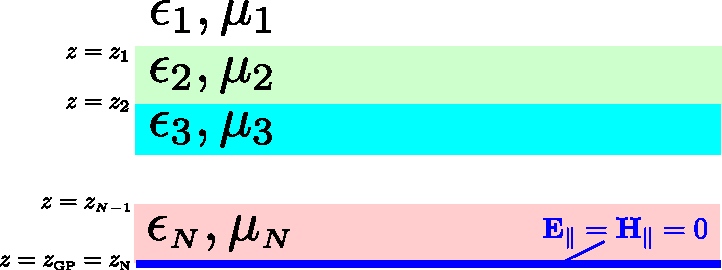
\includegraphics{MultilayerSubstrate.pdf}}
\caption{Geometry of the layered substrate.
The $n$th layer 
has relative permittivity and permeability $\epsilon_n,\mu_n$,
and its lower surface lies at $z=z_n$. The ground plane, if present,
lies at $z=z\subt{GP}.$
}
\label{SubstrateGeometryFigure}
\end{center}
\end{figure}
%####################################################################%

%%%%%%%%%%%%%%%%%%%%%%%%%%%%%%%%%%%%%%%%%%%%%%%%%%%%%%%%%%%%%%%%%%%%%%
%%%%%%%%%%%%%%%%%%%%%%%%%%%%%%%%%%%%%%%%%%%%%%%%%%%%%%%%%%%%%%%%%%%%%%
%%%%%%%%%%%%%%%%%%%%%%%%%%%%%%%%%%%%%%%%%%%%%%%%%%%%%%%%%%%%%%%%%%%%%%
\subsubsection*{Definition of the substrate DGF}

I will use the symbol $\vbGamma(\omega; \vb x\subt{D}, \vb x\subt{S})$
for the \textit{total} 6$\times$6 dyadic Green's function
relating time-harmonic fields at $\vb x\subt{D}$ to sources
at $\vb x\subt{S}$: thus,
if $\bmc S\equiv {\vb J \choose \vb M}$ is the 6-vector distribution
of free electric and magnetic currents in the presence of the 
substrate, then the 6-vector of
electric and magnetic fields $\bmc F\equiv {\vb E \choose \vb H}$
is given by 
%====================================================================%
$$ \bmc F(\vb x\subt{D}) = \int \vbGamma(\vb x\subt{D}, \vb x\subt{S})
   \cdot \bmc S(\vb x\subt{S}) d\vb x\subt{S}.
$$
%====================================================================%
The $6\times 6$ tensor $\vbGamma$ has a $2\times 2$ block structure:
%====================================================================%
\begin{subequations}
\begin{align} 
 \vbGamma
&=
 \left(\begin{array}{cc}
   \vbGamma\supt{EE} & \vbGamma\supt{EM} \\
   \vbGamma\supt{ME} & \vbGamma\supt{MM}
 \end{array}\right)
\intertext{with the $3\times 3$ subblocks defined by} 
\Gamma\supt{PQ}_{ij}(\omega, \vb x\subt{D}, \vb x\subt{S})&=
\left(\begin{parbox}{0.63\textwidth}
  { $i$-component of P-type field at $\vb x\subt{D}$ due to
    $j$-directed Q-type point current source at $\vb x\subt{S}$,
    all fields and sources having time dependence $\sim e^{-i\omega t}$
  } \end{parbox}\right)
\end{align}
\label{vbGammaDef}%
\end{subequations}
%====================================================================%
\paragraph{Homogeneous DGF}
In an infinite \textit{homogeneous} medium with relative permittivity
and permeability $\{\epsilon^r, \mu^r\}$, $\vbGamma$ reduces
to its homogeneous form, for which I will use the symbol
$\vbGamma^{0r}$ (where the $r$ index labels the medium, which
in this case will be one of the layers in
Figure \ref{SubstrateGeometryFigure}, i.e. $r\in\{1,2,\cdots,N\}$):
%====================================================================%
$$\vb x\subt{D},\vb x\subt{S} \in \text{infinite homogeneous medium } r
  \quad \Longrightarrow \quad 
   \vbGamma(\omega; \vb x\subt{D}, \vb x\subt{S})
= \vbGamma^{0r}(\omega; \vb x\subt{D}-\vb x\subt{S})
$$
where\footnote{Cf. Section 3 of the companion memo
``{\sc libscuff} implementation and Technical Details,''
\url{http://homerreid.github.io/scuff-em-documentation/tex/lsInnards.pdf}}
\numeq{vbGamma0Def}
{
 \vbGamma^{0r}(\omega, \vb r)
 \equiv
 \left(\begin{array}{cc}
   ik_r Z_0 Z^r \vb G(k_r,\vb r) & ik_r \vb C(k_r,\vb r)         \\[3pt]
  -ik_r \vb C(k_r,\vb r) & \frac{ik_r}{Z_0 Z^r} \vb G(k_r,\vb r) \\
 \end{array}\right)
}
$$ k_r \equiv \sqrt{\epsilon_0 \epsilon^r \mu_0 \mu^r}\cdot \omega,
   \quad 
   Z_0Z^r \equiv \sqrt\frac{\mu_0 \mu^r}{\epsilon_0 \epsilon^r},
$$
$$
   G_{ij}=\left(\delta_{ij} - \frac{1}{k^2}\partial_i \partial_j\right)
   \frac{e^{ik|\vb r|}}{4\pi|\vb r|},
   \quad
   C_{ij}=\frac{\varepsilon_{i\ell m}}{ik} \partial_\ell G_{m j}
$$
%====================================================================%
\paragraph{Inhomogeneous DGF}

On the other hand, in the presence of the
multilayered substrate the full DGF $\vbGamma$
receives corrections, which may be thought of as the
fields radiated by surface currents induced on the
interfacial surfaces of the substrate, and which I will 
denote by the symbol $\bmc G$:
%====================================================================%
\numeq{vbGammaCases}
{ \vbGamma(\vb x\subt{D}, \vb x\subt{S})
 = \bmc G(\vb x\subt{D}, \vb x\subt{S})
   +\begin{cases}
      \vbGamma^{0r}(\vb x\subt{D}-\vb x\subt{S})
      , &\vb x\subt{S} \in \text{layer r} 
      \\
      0,
      \qquad &\text{otherwise}
   \end{cases}
}
%====================================================================%
Like $\vbGamma$, $\bmc G$ is a 
$6\times 6$ matrix with a $2\times 2$ block structure:
%====================================================================%
\begin{align} 
 \bmc G(\omega; \vb x\subt{D}, \vb x\subt{S})
&=
 \left(\begin{array}{cc}
   \bmc G\supt{EE} & \bmc G\supt{EM} \\
   \bmc G\supt{ME} & \bmc G\supt{MM}
 \end{array}\right)
\label{ScriptGDef}
\intertext{with the $3\times 3$ subblocks defined by} 
\mc G\supt{PQ}_{ij}&=
\left(\begin{parbox}{0.83\textwidth}
  { $i$-component of P-type field at $\vb x\subt{D}$ due to
    surface currents on substrate interface layers induced
    by $j$-directed Q-type source at $\vb x\subt{S}.$
  } \end{parbox}\right)
\nonumber
\end{align}
{\sc libsubstrate} is a code for numerical computation of $\bmc G$.

%%%%%%%%%%%%%%%%%%%%%%%%%%%%%%%%%%%%%%%%%%%%%%%%%%%%%%%%%%%%%%%%%%%%%%
%%%%%%%%%%%%%%%%%%%%%%%%%%%%%%%%%%%%%%%%%%%%%%%%%%%%%%%%%%%%%%%%%%%%%%
%%%%%%%%%%%%%%%%%%%%%%%%%%%%%%%%%%%%%%%%%%%%%%%%%%%%%%%%%%%%%%%%%%%%%%
\subsubsection*{Organization of {\sc scuff-em} implementation and this memo}

The full-wave substrate implementation in {\sc scuff-em} consists of
multiple working parts that fit together in a somewhat modular fashion.

Roughly speaking, the computational problem may be divided into two parts:
%====================================================================%
\begin{description}
  \item[(a)] For given source and evaluation (or ``destination'')
             points $\{\vb x\subt{S}, \vb x\subt{D}\}$ at a given 
             angular frequency
             $\omega$ in the presence of a multilayer substrate,
             numerically compute the substrate DGF correction
             $\bmc G(\omega, \vb x\subt{D}, \vb x\subt{S})$.
             This task is independent of {\sc scuff-em}
             and is implemented by a standalone library
             called {\sc libsubstrate}, described in
             Section \ref{libSubstrateSection} of this memo.
  \item[(b)] For a {\sc scuff-em} geometry in the presence of a
             substrate, compute the substrate corrections to the BEM
             system matrix $\vb M$ and RHS vector $\vb v$,
             as well as the substrate corrections
             to post-processing quantities such as scattered fields.
             This is done by the file \texttt{Substrate.cc}
             in {\sc libscuff} and is described in 
             Section \ref{libscuffIntegrationSection} of this memo.
\end{description}
%====================================================================%

%####################################################################%
%####################################################################%
%####################################################################% 
\newpage
\section{{\sc libsubstrate:} Numerical computation of substrate Green's functions}
\label{libSubstrateSection}

Numerical evaluation of substrate contributions to
dyadic Green's functions is handled by a C++ library 
called {\sc libsubstrate}.
Although this library is packaged and distributed with {\sc scuff-em}
and depends on other support libraries in the {\sc scuff-em}
distribution, it is independent of the particular integral-equation
formulation implemented by {\sc libscuff}, and thus should be
of general utility beyond {\sc scuff-em}.

\subsection{Overview of computational strategy}
\label{libSubstrateStrategy}

{\sc libsubstrate} decomposes the problem of computing
$\bmc G$ into several logical steps, as follows:

\begin{description}
 \item[1.] Solve a linear system to obtain the Fourier-space
             representation $\bmc{\wt G(\vb q)}$. Here $\vb q=(q_x,q_y)$ is a
             2D Fourier variable. (Section \ref{GTwiddleSection}.)
 \item[2.] Reduce the two-dimensional integral over $\vb q$ to a
             one-dimensional integral over $|\vb q|\equiv q$.
             (Section \ref{gTwiddleSection}.)
 \item[3.] Evaluate the $q$ integral using established methods for
             evaluating Sommerfeld integrals.
             (Section \ref{SommerfeldSection}.)
\end{description}

%%%%%%%%%%%%%%%%%%%%%%%%%%%%%%%%%%%%%%%%%%%%%%%%%%%%%%%%%%%%%%%%%%%%%%
%%%%%%%%%%%%%%%%%%%%%%%%%%%%%%%%%%%%%%%%%%%%%%%%%%%%%%%%%%%%%%%%%%%%%%
%%%%%%%%%%%%%%%%%%%%%%%%%%%%%%%%%%%%%%%%%%%%%%%%%%%%%%%%%%%%%%%%%%%%%%
\newpage
\subsection{Computation of Fourier-space DGF $\bmc{\wt G}(\vb q)$}
\label{GTwiddleSection}

%####################################################################%
%####################################################################%
%####################################################################%
\begin{figure}[t]
\begin{center}
\resizebox{\textwidth}{!}{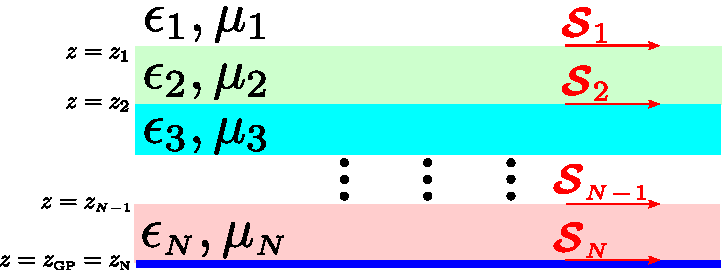
\includegraphics{MultilayerSubstrateWithSurfaceCurrents.pdf}}
\caption{Effective surface-current approach to treatment of
multilayer substrate. External field sources induce a distribution
of electric and magnetic surface currents $\bmc S_n={\vb K_n \choose \vb N_n}$
on the $n$th material interface, and the fields radiated by these
effective currents account for the disturbance presented by
the substrate.}
\label{SurfaceCurrentFigure}
\end{center}
\end{figure}
%####################################################################%
%####################################################################%
%####################################################################%
To compute the substrate correction to the fields of external sources,
I consider the effective tangential electric and magnetic
surface currents $\vb K$ and $\vb N$ induced on the interfacial 
layers by the external field sources 
(Figure \ref{SurfaceCurrentFigure}). This is the direct extension
to full-wave problems of the formalism I used in the electrostatic
case, and it comports well with the spirit of
surface-integral-equation methods.

More specifically, on the material interface layer at $z=z_n$
I have a four-vector surface-current density $\bmc S_n(\vbrho)$,
where $\vbrho=(x,y)$ and the components of $\bmc S$ are
%====================================================================%
\numeq{SnDef}
{ \bmc S_n(\vbrho)=
  \left(\begin{array}{c}
     K_x(\vbrho) \\ K_y(\vbrho) \\ N_x(\vbrho) \\ N_y(\vbrho)
  \end{array}\right).
}
%====================================================================%

\paragraph{Fields in layer interiors.} 
I will adopt the convention that the lower (upper) bounding surface
for each region is the positive (negative) bounding surface
for that region in the usual sense of {\sc scuff-em} regions and
surfaces (in which the sign of a \{surface,region\} pair $\{\mc S, \mc R\}$ 
is the sign with which surface currents on $\mc S$ contribute to
fields in $\mc R$).
Thus, at a point $\vb x=(\vbrho,z)$ in the interior of layer $n$
($z_{n-1} > z > z_n$), the six-vector of total fields
$\bmc F=\hbox{\scriptsize{
 $\left(\begin{array}{c} \vb E \\ \vb H\end{array}\right)$}}
$
reads
%====================================================================%
\numeq{Fn}
{  \bmc F_n(\vbrho, z)
  =
  - \vbGamma^{0n}(z_{n-1}) \star \bmc S_{n-1}
  + \vbGamma^{0n}(z_{n}) \star \bmc S_{n}
  + \bmc F\sups{ext}_n(\vbrho, z)
}
%====================================================================%
where $\bmc F\sups{ext}_n$
are the externally-sourced (incident) fields
due to sources in layer $n$, $\vbGamma^{0n}$ is the $6\times 6$ 
homogeneous dyadic Green's function for material layer $n$, 
and $\star$ is shorthand for the convolution operation
%====================================================================%
\numeq{ConvolutionDef}
{
``\bmc F(\vbrho, z) \equiv \vbGamma(z^\prime) \star \bmc S''
   \quad \Longrightarrow \quad 
    \bmc F(\vbrho,z) = 
    \int
      \vbGamma(\vbrho-\vbrho^\prime,z-z^\prime)\cdot \bmc S(\vbrho^\prime)
    d\vbrho^\prime
}
%====================================================================%
where the integral extends over the entire interfacial plane.
I will evaluate convolutions of this form using the
2D Fourier representation of $\vbGamma^{0n}$:
%====================================================================%
\begin{subequations}
\begin{align}
  \vbGamma^{0n}(\vbrho, z)
 &=
  \int \frac{d^2 \vb q}{(2\pi)^2}
  \wt{\vbGamma^{0n}}(\vb q, z) e^{i\vb q \cdot \vbrho}
\\
%--------------------------------------------------------------------%
   \wt{\vbGamma^{0n}}(\vb q, z)
&= \frac{1}{2}
   \left(\begin{array}{cc}
      -\frac{\omega \mu_0 \mu_n}{q_{zn}} \wt{\vb G}^\pm
    & +\wt{\vb C}^\pm 
    \\[5pt]
      -\wt{\vb C}^\pm
    & -\frac{\omega \epsilon_0 \epsilon_n}{q_{zn}} \wt{\vb G}^\pm
   \end{array}\right)e^{iq_z |z|}
\\[10pt]
%--------------------------------------------------------------------%
   \wt{\vb G}^\pm(\vb q, k)
&= \left(\begin{array}{ccc}
   1 & 0 & 0 \\[2pt] 0 & 1 & 0 \\[2pt] 0 & 0 & 1
   \end{array}\right)
   -
   \frac{1}{k^2}
   \left(\begin{array}{ccc}
    q_x^2    & q_xq_y       & \pm q_x q_z \\[2pt]
    q_y q_x  & q_y^2        & \pm q_y q_z \\[2pt]
 \pm q_z q_x  & \pm q_z q_y  & q_z^2 
   \end{array}\right)
\\[10pt]
%--------------------------------------------------------------------%
   \wt{\vb C}^\pm(\vb q, k)
&=
   \left(\begin{array}{ccc}
   0           & \mp 1     &    +q_y/q_z \\[2pt]
   \pm 1       & 0         &    -q_x/q_z \\[2pt]
  -q_y/q_z     & +q_x/q_z  &           0
  \end{array}\right)
\end{align}
\label{GFourier}
\begin{equation}
  k_n\equiv \sqrt{\epsilon_0 \epsilon_n \mu_0 \mu_n}\cdot \omega,
  \qquad 
  q_z \equiv \sqrt{k^2 - |\vb q|^2},
 \qquad 
  \pm = \text{sign } z.
\end{equation}
\end{subequations}
%====================================================================%
\noindent With this representation, convolutions like (\ref{ConvolutionDef})
become products in Fourier space:
%====================================================================%
\begin{align*}
\vbGamma (z^\prime)\star \bmc S=
 \bmc F(\vbrho, z)
&=\int \frac{d^2 \vb q}{(2 \pi)^2} \wt{\bmc F}(\vb q,z) e^{i\vb q \cdot \vbrho},
\qtq{with}
 \wt{\bmc F}(\vb q,z)=\wt{\vbGamma}(\vb q,z-z^\prime)\wt{\bmc S}(\vb q)
\end{align*}
%====================================================================%

\paragraph{Surface currents from incident fields.}

To determine the surface currents induced by given incident-field
sources, I apply boundary conditions.
The boundary condition at $z=z_n$ is that the tangential $\vb E, \vb H$
fields be continuous: in Fourier space, we have
%====================================================================%
\numeq{BCEquation}
{ \wt{\bmc F}_{\parallel}(\vb q, z=z_n^+)
 =\wt{\bmc F}_{\parallel}(\vb q, z=z_n^-)
}
The fields just \textbf{above} the interface $(z\to z_n^+)$ receive
contributions from three sources:
%====================================================================%
\begin{itemize}
 \item Surface currents at $z=z_{n-1}$, which contribute with
       a minus sign and via the Green's function for region $n$;
 \item Surface currents at $z=z_{n}$, which contribute with
       a plus sign and via the Green's function for region $n$; and
 \item external field sources in region $n$.
\end{itemize}
%====================================================================%
The fields just \textbf{below} the interface $(z=z_n^-)$ receive
contributions from three sources:
%====================================================================%
\begin{itemize}
 \item Surface currents at $z=z_{n}$, which contribute with
       a minus sign and via the Green's function for region $n+1$;
 \item Surface currents at $z=z_{n+1}$, which contribute with
       a plus sign and via the Green's function for region $n+1$; and
 \item external field sources in region $n+1$.
\end{itemize}
%====================================================================%
Then equation (\ref{BCEquation}) reads (temporarily omitting $\vb q$
arguments)
%====================================================================%
\begin{align*}
&
-\wt{\vbGamma^{0n}}_{\parallel}(z_n-z_{n-1})\cdot \wt{\bmc S}_{n-1}
+\wt{\vbGamma^{0n}}_{\parallel}(0^+) \cdot \wt{\bmc S}_{n}
+\wt{\bmc F}\sups{ext}_{n\parallel}(z_n)
\\
&\qquad=
-\wt{\vbGamma^{0,n+1}}{\parallel}(0^-) \cdot \wt{\bmc S}_{n}
+\wt{\vbGamma^{0,n+1}}{\parallel}(z_n-z_{n+1})\cdot \wt{\bmc S}_{n+1}
+\wt{\bmc F}\sups{ext}_{n+1\parallel}(z_n)
\end{align*}
or
%====================================================================%
\numeq{MSFSlice}
{
  \vb M_{n,n-1}  \cdot \wt{\bmc S}_{n-1}
 +\vb M_{n,n}    \cdot \wt{\bmc S}_{n}
 +\vb M_{n,n+1}  \cdot \wt{\bmc S}_{n+1}
 =  \wt{\bmc F}\sups{ext}_{n+1\parallel}(z_n)
   -\wt{\bmc F}\sups{ext}_{n\parallel}(z_n)
}
%====================================================================%
with the $4\times 4$ matrix blocks\footnote{The $4\times 4$ $\vb M$
blocks here have $2\times 2$ block structure:
%====================================================================%
\begin{align}
 \vb M_{n, n}
   &= \sum_{r\in \{n, n+1\}}
     \frac{1}{2}
     \left(\begin{array}{cc}
     -\frac{\omega\epsilon_r}{Z_0 q_{zr}}\vb g(k_r, \vb q)
   & 0
 \\
     0
   & -\frac{\omega\mu_r Z_0 }{q_{zr}}\vb g(k_r, \vb q)
   \end{array}\right)
\\
 \vb M_{n, n \pm 1}
   &= \frac{1}{2}
     \left(\begin{array}{cc}
     -\frac{\omega\epsilon_r}{Z_0 q_{zr}}\vb g(k_r, \vb q)
   & \vb c^\pm
 \\
     -\vb  c^\pm
   & -\frac{\omega\mu_r Z_0 }{q_{zn^*}}\vb g(k_r, \vb q)
     \end{array}\right)e^{iq_{zr}|z_n-z_{n\pm 1}|}
\end{align}
%====================================================================%
where I put
$  r \equiv  \begin{cases} n,   \qquad &\text{ for } \vb M_{n,n-1} \\
                           n+1, \qquad &\text{ for } \vb M_{n,n+1}
              \end{cases}.
$
and 
%====================================================================%
$$ \vb g(k; \vb q) =
   \vb 1 - \frac{\vb q\vb q^\top}{k^2},
   \qquad 
   \vb c^\pm
   =\left(\begin{array}{cc} 0 & \mp 1 \\ \pm 1 & 0 \end{array}\right)
$$}
%====================================================================%
%====================================================================%
\begin{subequations}
\begin{align}
  \vb M_{n,n-1} &= -\wt{\vbGamma^{0n}}_{\parallel}(z_n-z_{n-1}) 
\\
  \vb M_{n,n} &= +\wt{\vbGamma^{0n}}_{\parallel}(0^+)
                 +\wt{\vbGamma^{0,n+1}}_{\parallel}(0^-)
\\
  \vb M_{n,n+1} &= -\wt{\vbGamma^{0,n+1}}_{\parallel}(z_n-z_{n+1}) 
\end{align}
\label{MChunks}%
\end{subequations}
%====================================================================%
Writing down equation (\ref{MSFSlice}) equation for all $N$ dielectric
interfaces yields a $4N\times 4N$ 
system of linear equations, with triadiagonal $4\times 4$ block form,
relating the surface currents on all layers
to the external fields due to sources in all regions:
%====================================================================%
\numeq{Msf}{\vb M\cdot \vb s = \vb f}
%====================================================================%
where $\vb M$ is the $4N\times 4N$ block-tridiagonal matrix
(\ref{MChunks}) and where the $4N$-vectors $\vb s$, $\vb f$ read
%====================================================================%
$$ 
   \vb s=\left(\begin{array}{c}
   \wt{\bmc S}_1 \\ \wt{\bmc S}_2 \\ \wt{\bmc S}_3 \\ \vdots \\
   \wt{\bmc S}_N
   \end{array}\right),
\qquad 
   \vb f=\left(\begin{array}{c}
  -\wt{\bmc F}_{1\parallel}(z_1)
  +\wt{\bmc F}_{2\parallel}(z_1)
\\
  -\wt{\bmc F}_{2\parallel}(z_2)
  +\wt{\bmc F}_{3\parallel}(z_2)
\\
  -\wt{\bmc F}_{3\parallel}(z_3)
  +\wt{\bmc F}_{3\parallel}(z_4)
\\
  \vdots
\\
  -\wt{\bmc F}_{N-1,\parallel}(z_{N-1})
  +\wt{\bmc F}_{N\parallel}(z_{N-1})
   \end{array}\right).
$$
%====================================================================%
Solving (\ref{Msf}) yields the induced surface currents on all
layers in terms of the incident fields:
%====================================================================%
$$ \vb s = \vb W \cdot \vb f \qtq{where} \vb W\equiv \vb M^{-1} $$
%====================================================================%
or, more explicitly,
%====================================================================%
\numeq{sWf}
{
 \wt{\bmc S}_n = \sum_{m} W_{nm} \vb f_m
}
%====================================================================%

%====================================================================%
%====================================================================%
%====================================================================%
\subsubsection*{Surface currents induced by point sources}

For DGF computations the incident fields arise from
a single point source---say, a $j$-directed source
in region $s$.
Then the only nonzero length-$4$ blocks of the RHS vector in
(\ref{Msf}) are $\vb f_{s-1}, \vb f\subt{S}$ with components
($\ell=\{1,2,4,5\}$)
%====================================================================%
\numeq{fsm1fs}
 { \Big(\vb f_{s-1}\Big)_\ell = -\wt{\Gamma}_{\ell j}^{0s}( z_{s-1}-z\subt{S}),
   \qquad
   \Big(\vb f_{s}\Big)_\ell   = +\wt{\Gamma}_{\ell j}^{0s}(z\subt{S}-z\subt{S})
 }
%====================================================================%
and the surface currents on interface layer $n$ are obtained
by solving (\ref{sWf}):
%====================================================================%
\begin{align}
 \wt{\bmc S}_n 
&= \vb W_{n,s-1} \, \vb f_{s-1} + \vb W_{n,s} \, \vb f_{s}
\nn
&= \sum_{p=0}^1 (-1)^{p+1} \vb W_{n,s-1+p}
    \cdot
    \wt{\vbGamma^{0s}}_{\parallel, j}(z\subt{S}-z_{s-1+p})
\label{SWG}
\end{align}
%====================================================================%

%====================================================================%
%====================================================================%
%====================================================================%
\subsubsection*{Fields due to surface currents}

Given the surface currents induced by a $j$-directed point
source at $\vb x\subt{S}$, I evaluate the fields due to
these currents to get the substrate DGF contribution $\bmc G$.
If the evaluation point $\vb x\subt{D}$ lies in region $d$,
then the fields receive contributions from the surface currents
at $z_{d-1}$ and $z\subt{D}$, propagated by the homogeneous DGF
for region $d$:
%====================================================================%
\begin{align}
\wt{\bmc F}(z\subt{D}) 
&= -\wt{\vbGamma^{0d}}(z\subt{D} - z_{d-1}) \cdot \wt{\bmc S}_{d-1}
   +\wt{\vbGamma^{0d}}(z\subt{D} - z\subt{D})     \cdot \wt{\bmc S}_{d}
\nn
&= \sum_{q=0}^1  (-1)^{q+1}
   \wt{\vbGamma^{0d}}(z\subt{D} - z_{d+q-1}) \cdot \wt{\bmc S}_{d+q-1}
\label{FieldsFromInducedCurrents}\\
\intertext{(The minus sign in the first term arises because, in my convention,
surface currents on the upper surface of a region contribute to the fields
in that region with a minus sign). Inserting (\ref{SWG}), the $i$ component
here---which is the $ij$ component of the substrate DGF---is}
\wt{\mc G}_{ij}(z\subt{D},z\subt{S})
&= \sum_{p,q=0}^1 (-1)^{p+q}
   \wt{\vbGamma^{0d}}_{i,\parallel} (z\subt{D}-z_{d-1+q})
   \vb W_{d-1+q,s-1+p}
   \wt{\vbGamma^{0s}}_{\parallel, j} (z_{s-1+p} - z\subt{S}).
\label{ScriptGFourier}
\end{align}
%====================================================================%
The calculation of equation (\ref{ScriptGFourier}) is carried
out by the routine \texttt{GetGTwiddle} in {\sc libsubstrate}.

\subsection*{Green's functions for potentials}

In equation (\ref{FieldsFromInducedCurrents}) I am computing
the 6 components of the $\vb E$ and $\vb H$ fields produced
by the induced surface currents. If instead I compute the
\textit{potentials} produced by those currents I obtain a
slightly different Green's function. Thus, let
$\vb A\supt{E}, \Phi\supt{E}$ be the usual vector and scalar
potential of an electric-current source in a homogeneous region,
and let $\vb A\supt{M}, \Phi\supt{M}$ be their counterparts for 
magnetic-current sources, i.e. if the electric and magnetic
volume currents are $\vb J$ and $\vb M$ then
%%%%%%%%%%%%%%%%%%%%%%%%%%%%%%%%%%%%%%%%%%%%%%%%%%%%%%%%%%%%%%%%%%%%%%
\begin{subequations}
\begin{align}
 \vb A\supt{E}(\vb x\subt{D})
&= \mu
   \int \vb J (\vb x\subt{S}) G_0(\vb x\subt{DS})\,d\vb x\subt{S},
 \quad
 \Phi\supt{E}(\vb x\subt{D})
 = \frac{1}{i\omega \epsilon}
   \int \left(\nabla\cdot \vb J\right) G_0(\vb x\subt{DS}) d\vb x\subt{S}
\\
%--------------------------------------------------------------------%
 \vb A\supt{M}(\vb x\subt{D})
&= \epsilon
   \int \vb M (\vb x\subt{S}) G_0(\vb x\subt{DS})\,d\vb x\subt{S},
 \quad
 \Phi\supt{M}(\vb x\subt{D})
 = \frac{1}{i\omega \mu}
   \int \left(\nabla\cdot \vb M\right) G_0(\vb x\subt{DS}) d\vb x\subt{S}
\end{align}
\end{subequations}
%%%%%%%%%%%%%%%%%%%%%%%%%%%%%%%%%%%%%%%%%%%%%%%%%%%%%%%%%%%%%%%%%%%%%%
with $\vb x\subt{DS}\equiv \vb x\subt{D}-\vb x\subt{S}$ and
%%%%%%%%%%%%%%%%%%%%%%%%%%%%%%%%%%%%%%%%%%%%%%%%%%%%%%%%%%%%%%%%%%%%%%
\begin{align*}
 G_0(k; \vb r)
 &=\frac{e^{ik|\vb r|}}{4\pi|\vb r|}
  =\int\frac{d^2 \vb q}{(2\pi)^2} 
   \wt{G}_0(\vb q, z)e^{i\vb q\cdot \vbrho},
 \qquad \wt{G}_0=\frac{i}{2q_z}e^{iq_z|z|}.
\end{align*}
%%%%%%%%%%%%%%%%%%%%%%%%%%%%%%%%%%%%%%%%%%%%%%%%%%%%%%%%%%%%%%%%%%%%%%
I write

%%%%%%%%%%%%%%%%%%%%%%%%%%%%%%%%%%%%%%%%%%%%%%%%%%%%%%%%%%%%%%%%%%%%%%
%%%%%%%%%%%%%%%%%%%%%%%%%%%%%%%%%%%%%%%%%%%%%%%%%%%%%%%%%%%%%%%%%%%%%%
%%%%%%%%%%%%%%%%%%%%%%%%%%%%%%%%%%%%%%%%%%%%%%%%%%%%%%%%%%%%%%%%%%%%%%
\newpage
\subsection{Reduction of 2D Fourier integrals to 1D (Sommerfeld) integrals}
\label{gTwiddleSection}

The real-space DGF correction is the inverse Fourier transform of
(\ref{ScriptGFourier}):
%====================================================================%
\begin{align}
  \bmc G(\vbrho, z\subt{D}, z\subt{S})
&= \int \frac{d^2 \vb q}{(2\pi)^2}
  \wt{\bmc G}
      (\vb q; z\subt{D};z\subt{S}) e^{i\vb q \cdot \vbrho}
\nonumber
\intertext{or, in polar coordinates with 
           $(q_x,q_y)=(q\cos\theta_q, q\sin\theta_q),$
           $(\rho_x,\rho_y)=(\rho\cos\theta_\rho, \rho\sin\theta_\rho),$}
\bmc G(\vbrho)
&= \int_{0}^\infty \frac{q\,dq}{2\pi}
   \int_0^{2\pi} \frac{d \theta_q}{2\pi}
   \wt{\bmc G} (\vb q) e^{iq\rho \cos(\theta_q - \theta_\rho)}.
\label{q2DIntegral}
\end{align}
%====================================================================%
(Here and for much of this section I suppress $z\subt{D,S}$ arguments,
but one must remember that they are always there.\footnote{More specifically,
the ``$g$-like'' quantities
$\bmc G(\vbrho), \wt{\bmc G}(\vb q), \wt{g}(q), \wt{\mathfrak{g}}(q,\rho),$
and $\mathfrak{g}(\rho)$ all depend on $z\subt{S,D}$,
but the matrix-valued functions $\vbLambda_n(\theta)$ do not.})
The goal of this section is to integrate out the angular variable $\theta_q$
to reduce the 2D integral over $\vb q$
to a 1D integral over $q=|\vb q|$. In abbreviated form this 
proceeds as follows:
%====================================================================%
\begin{enumerate}
 \item Separate variables by writing $\wt{\bmc G}(\vb q)$ as a sum of
       products of $\theta_{q}$-independent scalar functions
       $\wt g(q)$ times $q-$independent matrix-valued functions
       $\vbLambda(\theta_{q})$ (Section \ref{wtGDecomposition}):
       $$ \wt{\bmc G}(\vb q)=\sum_{n=1}^{18}
          \wt{g}^{(n)}(q) \vbLambda^{(n)}(\theta_{q})
       $$
 \item Evaluate integrals over $\theta_{q}$ analytically to yield
       Bessel functions $J_\nu(q\rho)$ multiplying $q$-independent
       matrix-valued functions $\vbLambda(\theta_{\rho})$
       (Section \ref{qThetaIntegral}).
       After this step (\ref{q2DIntegral}) reads
       \numeq{ScriptGgfrak}
        { \bmc G(\vbrho)
           = \sum_{m=1}^{22}
             \underbrace{
               \left[ \int_{0}^\infty \wt{\mathfrak{g}}^{(m)}(q,\rho)\,dq\right]
                        }_{\mathfrak{g}^{(m)}(\rho)}
             \vbLambda^{(m)}(\theta_{\rho})
        }
       where the $\wt{\mathfrak{g}}(q,\rho)$ functions are linear combinations
       of the $\wt{g}(q)$ functions times Bessel functions in $q\rho$
       and other factors.
 \item Evaluate the remaining integrals over $q$ numerically
       using sophisticated tricks for evaluating Sommereld
       integrals (Section \ref{SommerfeldIntegral}).
\end{enumerate}
%====================================================================%

%=================================================
%=================================================
%=================================================
\subsubsection{Factor $\wt{\bmc G}$ into $q$-independent and $\theta_{\vb q}$-independent terms}
\label{wtGDecomposition}

I begin by noting that $\wt{\bmc G}(\vb q)$ may be decomposed as a sum
of scalar functions of $q=|\vb q|$ times $q$-independent
matrix-valued functions of $\theta_{\vb q}:$
%====================================================================%
\numeq{gTwiddleDef}
{
  \wt{\bmc G}(\vb q)=\sum_{n=1}^{18}
  \wt{g}^{(n)}(q) \vbLambda^{(n)}(\theta_{\vb q})
}
%====================================================================%
For example, the upper two quadrants read
%====================================================================%
\begin{align*}
 \wt{\bmc G\supt{EE}}(\vb q)
 = &\wt{g}\supt{EE0$\parallel$}(q)
    \underbrace{ \left(\begin{array}{ccc}
                       1 & 0 & 0 \\ 
                       0 & 1 & 0 \\ 
                       0 & 0 & 0 \\ 
                 \end{array}\right)
               }_{\vbLambda^{0\parallel}}
  + \wt{g}\supt{EE0$z$}(q)
    \underbrace{ \left(\begin{array}{ccc}
                       0 & 0 & 0 \\ 
                       0 & 0 & 0 \\ 
                       0 & 0 & 1 \\ 
                 \end{array}\right)
               }_{\vbLambda^{0z}}
\\[10pt]
%--------------------------------------------------------------------%
 + &\wt{g}\supt{EE1}(q)
    \underbrace{ \left(\begin{array}{ccc}
                       0 & 0 & \cos\theta_{\vb q} \\ 
                       0 & 0 & \sin\theta_{\vb q} \\ 
                       0 & 0 & 0
                 \end{array}\right)
               }_{\vbLambda^{1}(\theta_{\vb q})}
 +  \wt{g}\supt{EE1$\top$}(q)
    \underbrace{ \left(\begin{array}{ccc}
                       0 & 0 & 0 \\
                       0 & 0 & 0 \\
                       \cos\theta_{\vb q} & \sin\theta_{\vb q} & 0
                 \end{array}\right)
               }_{\vbLambda^{1\top}(\theta_{\vb q})}
\\[10pt]
%--------------------------------------------------------------------%
  +&\wt{g}\supt{EE2}(q)
    \underbrace{
   \left(\begin{array}{ccc}
    \cos^2\theta_{\vb q}  & \cos\theta_{\vb q} \sin\theta_{\vb q} & 0 \\
    \cos\theta_{\vb q} \sin\theta_{\vb q} & \sin^2\theta_{\vb q}  & 0 \\
    0                     & 0                    & 0 
   \end{array}\right)
               }_{\vbLambda^{2}(\theta_{\vb q})}
\\[20pt]
%--------------------------------------------------------------------%
 \wt{\bmc G\supt{EM}}(\vb q)
 = &\wt g\supt{EM0$\parallel$}(q)
    \underbrace{ \left(\begin{array}{ccc}
                       0 & 1 & 0 \\ 
                      -1 & 0 & 0 \\ 
                       0 & 0 & 0 
                 \end{array}\right)
               }_{\vbLambda^{0\times}}
  +\wt g\supt{EM2}(q)
   \underbrace{
   \left(\begin{array}{ccc}
    \cos\theta_{\vb q} \sin\theta_{\vb q} & \sin^2\theta_{\vb q} & 0 \\
    -\cos^2\theta_{\vb q} & -\cos\theta_{\vb q} \sin\theta_{\vb q} & 0 \\
    0                     & 0                    & 0 
   \end{array}\right)
              }_{\vbLambda^{2\times}}
\\[10pt]
%--------------------------------------------------------------------%
  + &\wt g\supt{EM1}(q)
   \underbrace{
    \left(\begin{array}{ccc}
    0 & 0 & -\sin\theta_{\vb q} \\
    0 & 0 & +\cos\theta_{\vb q} \\
    0 & 0 & 1
   \end{array}\right)
              }_{\vbLambda^{1\times}}
  + \wt g\supt{EM1$\top$}(q)
   \underbrace{
    \left(\begin{array}{ccc}
    0 & 0 & 0 \\
    0 & 0 & 0 \\
   -\sin\theta_{\vb q} & \cos\theta_{\vb q} & 1
   \end{array}\right)
              }_{\vbLambda^{1\times\top}}
\end{align*}
where the $\top$ superscript indicates matrix transpose.
The expressions for $\wt{\bmc G}\supt{ME}$ and $\wt{\bmc G}\supt{MM}$
are similar, involving the same $\Lambda$ matrices with different
$\wt{g}$ prefactors.

%=================================================
%=================================================
%=================================================
\subsubsection{Evaluate $\theta_{\vb q}$ integrals}
\label{qThetaIntegral}

%%%%%%%%%%%%%%%%%%%%%%%%%%%%%%%%%%%%%%%%%%%%%%%%%%%%%%%%%%%%%%%%%%%%%
%%%%%%%%%%%%%%%%%%%%%%%%%%%%%%%%%%%%%%%%%%%%%%%%%%%%%%%%%%%%%%%%%%%%%
%%%%%%%%%%%%%%%%%%%%%%%%%%%%%%%%%%%%%%%%%%%%%%%%%%%%%%%%%%%%%%%%%%%%%
\begin{figure}
$$
 \frac{1}{2\pi} 
 \int_0^{2\pi} e^{i q \rho \cos(\theta_q -\theta_\rho)}
 \left\{\begin{array}{c}
 1 \\[5pt]
 \cos\theta_q \\[5pt]
 \sin\theta_q \\[5pt]
 \cos^2\theta_q \\[5pt]
 \cos\theta_q \sin\theta_q \\[5pt]
 \sin^2\theta_q \\
 \end{array}\right\}
 d\theta_q 
%--------------------------------------------------------------------%
= \left\{ \begin{array}{l}
    J_0 (q\rho)                           \\[5pt]
    i J_1(q\rho) \cos \theta_\rho          \\[5pt]
    i J_1(q\rho) \sin \theta_\rho          \\[5pt]
    - J_2(q\rho) \cos^2\theta_\rho + \frac{J_1(q\rho)}{q\rho} \\[5pt]
    -J_2(q\rho) \cos\theta_\rho \sin \theta_\rho              \\[5pt]
    - J_2(q\rho) \sin^2 \theta_\rho + \frac{J_1(q\rho)}{q\rho} 
  \end{array}\right\},
$$
\caption{Table of integrals used to reduce 2D integrals over $\vb q$ to
         1D integrals over $|q|$.}
\label{BesselIntegralTable}
\end{figure}
%%%%%%%%%%%%%%%%%%%%%%%%%%%%%%%%%%%%%%%%%%%%%%%%%%%%%%%%%%%%%%%%%%%%%
%%%%%%%%%%%%%%%%%%%%%%%%%%%%%%%%%%%%%%%%%%%%%%%%%%%%%%%%%%%%%%%%%%%%%
%%%%%%%%%%%%%%%%%%%%%%%%%%%%%%%%%%%%%%%%%%%%%%%%%%%%%%%%%%%%%%%%%%%%%

Using Table \ref{BesselIntegralTable}, the $\theta_{\vb q}$ integral
in (\ref{q2DIntegral}) may be evaluated analytically to yield
Bessel-function factors $J_\nu(q\rho)$ $(\nu\in\{0,1,2\})$
times $\vbLambda$ matrices, now evaluated at $\theta_{\vbrho}$. For
example, one term in the expansion of $\bmc G(\vbrho)$ is
%====================================================================%
\begin{align*}
& \int_0^\infty \frac{q dq}{2\pi} \wt{g}\supt{EE1}(q)
  \underbrace{
  \int_0^{2\pi} \frac{d\theta_q}{2\pi}
                \vbLambda\supt{1}(\theta_q)e^{iq\rho\cos(\theta_q-\theta_\rho)}
             }_{iJ_1(q\rho)\vbLambda^1(\theta_\rho)}
\\
&\qquad= \underbrace{
   \left\{\int_0^\infty \, dq
   \underbrace{
   \left[\frac{q}{2\pi} \wt{g}\supt{EE1}(q)\cdot iJ_1(q\rho)\right]
              }_{\wt{\mathfrak g}\supt{EE1}(q,\rho)}
   \right\}}_{\mathfrak{g}\supt{EE1}(\rho)}
   \vbLambda^1(\theta_\rho)
\end{align*}
%====================================================================%
The second line here defines some new symbols:
$\wt{\mathfrak{g}}$ are functions of $q$ and $\rho$
defined as products of $\wt{g}(q)$ factors times $J_\nu(q\rho)$
factors and other factors, while $\mathfrak{g}$ are
functions of $\rho$ obtained by integrating out the $q$ dependence
of $\mathfrak{g}(q,\rho)$.
The full set of rules defining the $\wt{\mathfrak{g}}$ is
%====================================================================%
\begin{subequations}
\begin{align}
  \wt{\mathfrak{g}}\supt{EE0$\parallel$}(q,\rho)
&\equiv\frac{q}{2\pi}\left[    \wt{g}\supt{EE0$\parallel$}(q) J_0(q\rho)
                       +  \wt{g}\supt{EE2}(q) \frac{J_1(q\rho)}{q\rho}
               \right]
\\
  \wt{\mathfrak{g}}\supt{EE0z}(q,\rho)
&\equiv\frac{q}{2\pi}\wt{g}\supt{EE0z}(q) J_0(q\rho)
\\
  \wt{\mathfrak{g}}\supt{EE1}(q,\rho)
&\equiv i\frac{q}{2\pi}\wt{g}\supt{EE1}(q) J_1(q\rho)
\\
  \wt{\mathfrak{g}}\supt{EE1$\top$}(q,\rho)
&\equiv i\frac{q}{2\pi}\wt{g}\supt{EE1$\top$}(q) J_1(q\rho)
\\
  \wt{\mathfrak{g}}\supt{EE2}(q,\rho)
&\equiv-\frac{q}{2\pi}\wt{g}\supt{EE2}(q) J_2(q\rho)
\\
  \wt{\mathfrak{g}}\supt{EM0$\parallel \times$}(q,\rho)
&\equiv\frac{q}{2\pi}\left[    \wt{g}\supt{EM0$\parallel$}(q) J_0(q\rho)
                       +  \wt{g}\supt{EM2}(q) \frac{J_1(q\rho)}{q\rho}
                 \right]
\\
  \wt{\mathfrak{g}}\supt{EM1$\times$}(q,\rho)
&\equiv i\frac{q}{2\pi}\wt{g}\supt{EM1A}(q) J_1(q\rho)
\\
  \wt{\mathfrak{g}}\supt{EM1$\times\top$}(q,\rho)
&\equiv i\frac{q}{2\pi}\wt{g}\supt{EM1B}(q) J_1(q\rho)
\\
  \wt{\mathfrak{g}}\supt{EM2$\times$}(q,\rho)
&\equiv-\frac{q}{2\pi}\wt{g}\supt{EM2}J_2(q\rho)
\end{align}
\label{wtgFrakDef}%
\end{subequations}
%====================================================================%

%=================================================
%=================================================
%=================================================
\subsubsection{Evaluate Sommerfeld integrals over $q$}
\label{SommerfeldIntegral}

Assembling the above pieces, the substrate DGF correction $\bmc G$
is a sum of 22 terms:\footnote{This tally treats the integrals
of the two integrand terms on the RHS of (\ref{wtgFrakDef}a) as two separate
integrals [and similarly for (\ref{wtgFrakDef}f) and the corresponding
equations for the ME and MM quadrants]. If the terms
are lumped together then the number of distinct $\mathfrak{g}$ functions
is 18.}
%====================================================================%
\begin{align}
  \bmc G(\rho) &= \sum_{m=1}^{22} \mathfrak{g}^{(m)}(\rho) \vbLambda^{(m)}(\theta_\rho),
\nonumber
\intertext{where the $\mathfrak{g}^{(m)}(\rho)$ functions are defined by
           Sommerfeld integrals:}
  \mathfrak{g}^{(m)}(\rho)
 &\equiv\int_0^\infty \wt{\mathfrak{g}}^{(m)}(q,\rho) \, dq.
\label{frakgDef}
\end{align}
  
%====================================================================%

%####################################################################%
%####################################################################%
%####################################################################%
\newpage
\section{{\sc scuff-em} integration: Substrate contributions to
         BEM matrix and RHS vector}
\label{libscuffIntegrationSection}

\subsection{Fields of individual basis functions}

%====================================================================%
\begin{align*}
 \bmc G\supt{EE}
&=
\end{align*}
%====================================================================%

\subsection{SIE matrix elements: Panel-panel integrals}

If $\mc S_\alpha, S_\beta$ are two \texttt{RWGSurfaces} 
exposed to the outermost (ambient) region in a {\sc scuff-em}
geometry, then the elements of the SIE matrix elements corresponding
to any pair of basis functions
$\{\vb b_a\in \mc S_\alpha, \vb b_b\in \mc S_\beta\}$ receive
corrections of the form
%====================================================================%
\begin{align}
   \Delta M\supt{PQ}_{ab}
 &=\Vmv{\vb b_a}{\bmc G\supt{PQ}}{\vb b_b}
\nn
&\equiv \iint
    \vb    b_a(\vb x_a)
    \cdot \bmc G\supt{PQ}(\vb x_a, \vb x_b)
    \cdot \vb b_b(\vb x_b)
    \,d\vb x_b 
    \,d\vb x_a 
\label{MPQabDef}
\end{align}
%====================================================================%
I will consider two different approaches for evaluating the
panel-panel integrals\footnote{I refer to 4-dimensional
integrals like (\ref{MPQabDef}) as ``panel-panel integrals'' because
they are a sum of contributions of integrals over pairs of flat
triangular panels.} here:
%====================================================================%
\begin{enumerate}
 \item The \textit{spectral inner} approach: In this case I simply evaluate
       the panel-panel cubature in (\ref{MPQabDef}), with values of
       $\bmc G$ at each cubature point computed via the methods
       of {\sc libsubstrate} as described in the previous section
       (possibly accelerated via interpolation tables).
       I call this the ``spectral inner'' method because in this case 
       the $q$ integral in the definition of $\bmc G$
       is the innermost of 3 integrals. Indeed, inserting equation
       (\ref{ScriptGgfrak}) we have
%====================================================================%
\begin{align}
\Delta M\supt{PQ}_{ab}
&\equiv \iint
    \vb    b_a(\vb x_a)
    \left\{ \sum \mathfrak{g}^{(m)}(\rho) \vbLambda^{(m)}(\theta_\rho) \right\}
    \vb b_b(\vb x_b)
    \,d\vb x_b \,d\vb x_a
\nonumber
\intertext{[where $\vbrho=(\vb x_a-\vb x_b)_\parallel=
           (\rho\cos \theta_\rho, \rho\sin \theta_\rho)$].
           Recalling the definition (\ref{frakgDef}), this is a sum
           of triple integrals:
          }
&\equiv \iint
    \vb    b_a(\vb x_a)
    \left\{ \sum\left[\int_0^\infty \wt{\mathfrak{g}}^{(m)}(q,\rho)dq\right]
                     \vbLambda^{(m)}(\theta_\rho) \right\}
     \cdot \vb b_b(\vb x_b)
    \,d\vb x_b \,d\vb x_a.
 \label{DeltaMSpectralOuter}
\end{align}

\item The \textit{spectral outer} approach: In this case I rearrange the
order of integration in (\ref{DeltaMSpectralOuter}) so that the $q$ integral
is the \textit{outermost} integral, with an integrand defined for each $q$
by a panel-panel integral involving the spectral-domain GF:
%====================================================================%
\begin{align}
\Delta M\supt{PQ}_{ab}
&= \int_0^\infty \left\{
    \iint \vb b_a(\vb x_a)
      \Big[ \sum \wt{\mathfrak{g}}^{(m)}(q,\rho) \vbLambda^{(m)}(\theta_\rho) 
      \Big]
          \vb b_b(\vb x_b)
    \,d\vb x_b \,d\vb x_a\right\} dq
 \label{DeltaMSpectralOuter}
\end{align}
%====================================================================%
\end{enumerate}

\begin{align*}
 \mc G_{ij}\supt{EE}
&=\delta_{ij}
\end{align*}
%A\begin{align*}
%\Vmv{\vb b_\alpha}{\vbGamma_0}{\vb b_\beta}
%&
%\end{align*}

%####################################################################%
%####################################################################%
%####################################################################%
\newpage
\section{Metal-on-Insulator geometries}

\begin{align*}
 \vb E &= iw \vb A - \nabla \phi
\\
              &= iw\mu G_0\star \vb J 
                 - \frac{1}{i\omega \epsilon}\nabla G_0\star \vbrho
\end{align*}

\begin{align*}
 \wt G\supt{$A$pp}
 &= \frac{1}{2\pi} q J_0(q\rho)\zeta\supt{App}
\\
 \wt G\supt{$A$pz}
 &= -\frac{1}{2\pi}(\epsilon_r-1) q^2 J_1(q\rho)\zeta\supt{Apz}
\\
 \wt G\supt{$\Phi$}
 &= \frac{1}{2\pi} \rho J_0(q\rho)\zeta\supt{$\Phi$}
\end{align*}

\begin{align*}
\zeta\supt{App}&=
 \displaystyle{
 \frac{1}{D\supt{TE}}\times
  \begin{cases} e^{-u_0 z} \\ \frac{\sinh u(z+h)}{\sinh uh} \end{cases}
              }
\\
\zeta\supt{Apz}&=
 \displaystyle{
 \frac{1}{D\supt{TE}D\supt{TM}}\times
 \begin{cases} e^{-u_0 z} \\ \frac{\cosh u(z+h)}{\cosh uh} \end{cases}
              }
\\
\zeta\supt{$\Phi$}&=
 \frac{N}{D\supt{TE}D\supt{TM}}\times
 \begin{cases} e^{-u_0 z} \\
               \frac{\sinh u(z+h)}{\sinh uh}
\end{cases}
\end{align*}

$$ \frac{N}{D\subt{TE}D\subt{TM}}\xrightarrow{u \to u_0}
   \frac{1-e^{-2u_0 h}}{u_0(\epsilon+1)}
   \sum_{n=0}^\infty \Big[-\eta e^{-2u_0 h}\Big]^n
$$

%\begin{align*}
%  \wt{G^\phi} \xrightarrow{u \to u_0}
%  \frac{1}{4\pi}q J_0(q\rho}
%\end{align*}

%####################################################################%
%####################################################################%
%####################################################################%
\newpage
\section{Unit-test framework}

The {\sc libsubstrate} standalone library comes with
a unit-test suite to test core functionality related
to calculation of substrate DGFs. Separately, the
unit-test suite for {\sc libscuff} includes tests
to check the integration of {\sc libsubstrate} 
into {\sc libscuff}.

\subsection{{\sc libsubstrate} unit tests}

\subsubsection{\texttt{tGTwiddle}}

The unit-test code \texttt{tGTwiddle.cc} tests that the full
Fourier-space DGF $\wt \vbGamma(\vb q, z\subt{D}, z\subt{S})$ satisfies the appropriate
boundary conditions at each layer of the layered substrate, namely
%====================================================================%
\numeq{tgTwiddleCondition1}
{ C^+(\text{P},i,\ell) \wt{\Gamma}\supt{PQ}_{ij}(\vb q, z_\ell+\eta, z\subt{S})
   C^-(\text{P},i,\ell) \wt{\Gamma}\supt{PQ}_{ij}(\vb q, z_\ell-\eta, z\subt{S})
}
%====================================================================%
where
%====================================================================%
$$ C^\pm(P, i, \ell)=
   \begin{cases}
    1, \qquad                 &i \in \{x,y\} \\
    \epsilon_\ell^\pm, \qquad &i=z, P=E \\
    \mu_\ell^\pm,      \qquad &i=z, P=H
   \end{cases}
$$
%====================================================================%
where $\{\epsilon,\mu\}_\ell^\pm$ are the
material properties for the layer above/below $z_\ell$, i.e.
(Figure \ref{MultilayerSubstrate.pdf})
%====================================================================%
$$ \{\epsilon_\ell, \mu_\ell\}^+ = \{\epsilon_\ell, \mu_\ell\},
   \qquad
   \{\epsilon_\ell, \mu_\ell\}^- = \{\epsilon_{\ell+1}, \mu_{\ell+1}\}.
$$
%====================================================================%
If a ground plane is present, we have the additional condition
%====================================================================%
\numeq{tgTwiddleCondition2}
{\wt{\Gamma}\supt{PQ}_{ij}(q,z\subt{GP},z\subt{S})=0 \qtq{for} i\in \{x,y\}.}
%====================================================================%
Conditions (\ref{tgTwiddleCondition1}) and (\ref{tgTwiddleCondition2})
must hold \textit{independently} of the indices $\text{Q}\in\{\text{E},\text{H}\}$
and $j\in\{1,2,3\}$ and of the values of $\vb q$ and $z\subt{S}$.

%%%%%%%%%%%%%%%%%%%%%%%%%%%%%%%%%%%%%%%%%%%%%%%%%%%%%%%%%%%%%%%%%%%%%%
%%%%%%%%%%%%%%%%%%%%%%%%%%%%%%%%%%%%%%%%%%%%%%%%%%%%%%%%%%%%%%%%%%%%%%
%%%%%%%%%%%%%%%%%%%%%%%%%%%%%%%%%%%%%%%%%%%%%%%%%%%%%%%%%%%%%%%%%%%%%%
\appendix
\newpage
\section{Symbols and indices used in this document}

%=================================================
%=================================================
%=================================================
\subsection{Symbols}

%====================================================================%
\renewcommand{\arraystretch}{1.5}
\begin{tabular}{|c|c|l|}\hline
\textbf{Symbol} & \textbf{Arguments} & \textbf{Description} \\\hline
   $\bmc F$
&  $\vb r$, geometry
&  \parbox{0.75\textwidth}
   { Field six-vector $\bmc F={\vb E \choose \vb H}$ }
\\\hline%--------------------------------------------------------------------%
   $\bmc C$
&  $\vb r$, geometry
&  \parbox{0.75 \textwidth}
    { Current six-vector $\bmc C={\vb J \choose \vb M}$ or
                         $\bmc C={\vb K \choose \vb N}$
    }
\\\hline%--------------------------------------------------------------------%
   $\vbGamma$
&  $\vbrho,z\subt{D},z\subt{S},\omega$, geometry
& Full (bare+scattered) $6\times 6$ dyadic Green's function,
  $\bmc F=\vbGamma \star \bmc C$
\\\hline%--------------------------------------------------------------------%
   $\vbGamma^{0r}$
&  $\vbrho,z\subt{D},z\subt{S},\omega,\epsilon^r,\mu^r$
& Bare (homogeneous) $6\times 6$ dyadic Green's function in region $r$
\\\hline%--------------------------------------------------------------------%
   $\bmc G$
&  $\vbrho,z\subt{D},z\subt{S},\omega$, geometry
& Scattering contribution to $\vbGamma$
  ($\vbGamma=\vbGamma^{0r} + \bmc G$)
\\\hline%--------------------------------------------------------------------%
   $\bmc P$
&  $\vb r$, geometry
&  \parbox{0.75\textwidth}
   { Potential eight-vector
      $\bmc P=\left(\begin{array}{c} \vb A\supt{E} \\[-6pt] \Phi\supt{E} \\[-6pt]
                                     \vb A\supt{M} \\[-6pt] \Phi\supt{M}
               \end{array}
         \right)
      $
    }
\\\hline%--------------------------------------------------------------------%
   $\bmc S$
&  $\vb r$, geometry
& \parbox{0.75 \textwidth}
    { Source eight-vector
      $\bmc S=\left(\begin{array}{c} \vb J \\[-6pt] \rho\supt{E} \\[-6pt]
                                     \vb M \\[-6pt] \rho\supt{M}
               \end{array}
         \right)
      $
    }
\\\hline%--------------------------------------------------------------------%
   $\boldsymbol{\Lambda}$
&  $\vbrho,z\subt{D},z\subt{S},\omega$, geometry
& Full (bare+scattered) $8\times 8$ dyadic Green's function,
  $\bmc P=\boldsymbol{\Pi} \star \bmc S$
\\\hline%--------------------------------------------------------------------%
   $\boldsymbol{\Lambda}^{0r}$
&  $\vbrho,z\subt{D},z\subt{S},\omega$, geometry
& Bare (homogeneous) $8\times 8$ dyadic Green's function
  for region $r$
\\\hline%--------------------------------------------------------------------%
   $\bmc L$
&  $\vbrho,z\subt{D},z\subt{S},\omega$, geometry
& Scattering contribution to $\vbLambda$
  ($\vbLambda=\vbLambda^{0r} + \bmc L$)
\\\hline%--------------------------------------------------------------------%
\end{tabular}
\renewcommand{\arraystretch}{1.0}
%====================================================================%

%=================================================
%=================================================
%=================================================
\subsection{Indices}

%====================================================================%
\renewcommand{\arraystretch}{1.5}
\begin{tabular}{|c|c|c|}\hline
\textbf{Index} & \textbf{Range} & \textbf{Significance} 
\\\hline
  $i,j$
& $\{1,2,3\}$
& Cartesian directions $x,y,z$
\\\hline%--------------------------------------------------------------------%
  $I,J$
& $\{1,2,3,4,5,6\}$
& \parbox{0.75\textwidth}
    { \medskip
      Electric/magnetic field/current components
     \begin{center}
     \begin{tabular}{|c|c|}\hline
       1,2,3 & $E_{x,y,z}$, $J_{x,y,z}$, $K_{x,y,z}$ \\\hline
       4,5,6 & $H_{x,y,z}$, $M_{x,y,z}$, $N_{x,y,z}$ \\\hline
     \end{tabular}
     \end{center}
    }
\\\hline%--------------------------------------------------------------------%
  $\mu,\nu$
& $\{1,2,3,4,5,6,7,8\}$
& \parbox{0.75\textwidth}
    {\medskip 
      Electric/magnetic potential/source components
     \begin{center}
     \begin{tabular}{|c|c|}\hline
       1,2,3 & $A\supt{E}_{x,y,z}$, $J_{x,y,z}$, $K_{x,y,z}$  \\\hline
       4     & $\Phi\supt{E}$, $\rho\supt{E}$, $\sigma\supt{E}$ \\\hline
       5,6,7 & $A\supt{M}_{x,y,z}$, $M_{x,y,z}$, $N_{x,y,z}$  \\\hline
       8     & $\Phi\supt{M}$, $\rho\supt{M}$, $\sigma\supt{M}$ \\\hline
     \end{tabular}
     \end{center}
    }
\\\hline
\end{tabular}
\renewcommand{\arraystretch}{1.0}
%====================================================================%

%%%%%%%%%%%%%%%%%%%%%%%%%%%%%%%%%%%%%%%%%%%%%%%%%%%%%%%%%%%%%%%%%%%%%%
%%%%%%%%%%%%%%%%%%%%%%%%%%%%%%%%%%%%%%%%%%%%%%%%%%%%%%%%%%%%%%%%%%%%%%
%%%%%%%%%%%%%%%%%%%%%%%%%%%%%%%%%%%%%%%%%%%%%%%%%%%%%%%%%%%%%%%%%%%%%%
\newpage
\section{$8\times 8$ Dyadic Green's Functions}

The usual $6\times 6$ dyadic Green's function $\vbGamma$
operates on a six-vector of currents to yield a six-vector
of fields. It is convenient to consider a slightly different
object that operates on an \textit{eight}-vector of sources
to yield an \textit{eight}-vector of potentials.

In the presence of magnetic currents, the usual (electric-current-sourced)
vector and scalar potentials $\vb A\supt{E},\Phi\supt{E}$,
are joined by their magnetic-current-sourced counterparts
$\vb A\supt{M},\Phi\supt{M}$, which are related to the fields
according to
%====================================================================%
\begin{align*}
 \vb E &=    i\omega \mu \vb A\supt{E}
           - \frac{1}{i\omega \epsilon}\nabla\Phi\supt{E}
           - \nabla \times \vb A\supt{M}
\\
 \vb M &=   \nabla \times \vb A\supt{E}
           + i\omega \epsilon \vb A\supt{M}
           - \frac{1}{i\omega \mu}\nabla\Phi\supt{M}.
\end{align*}
%====================================================================%
In a homogeneous region, the potentials\footnote{Note that my $\Phi\supt{E,M}$
are $i\omega$ times the actual scalar potentials due to the charge
distributions associated with currents $\vb J, \vb M$.}
produced by given source distributions $\{\vb J, \vb M\}$ are
%====================================================================%
\begin{align*}
 \vb A\supt{E}(\vb x\subt{D})
 &= \int G_0(\vb x\subt{D}-\vb x\subt{S}) \vb J(\vb x\subt{S}) \, d\vb x\subt{S},
\qquad \,\,\,\,
 \Phi\supt{E}(\vb x\subt{D})
 = \int G_0(\vb x\subt{D}-\vb x\subt{S}) \big[\nabla \cdot \vb J\big]
    \, d\vb x\subt{S}
\\
 \vb A\supt{M}(\vb x\subt{D})
 &= \int G_0(\vb x\subt{D}-\vb x\subt{S}) \vb M(\vb x\subt{S}) \, d\vb x\subt{S},
\qquad 
 \Phi\supt{M}(\vb x\subt{D})
 = \int G_0(\vb x\subt{D}-\vb x\subt{S}) \big[\nabla \cdot \vb M\big]
    \, d\vb x\subt{S}
\end{align*}
%====================================================================%
where 
%====================================================================%
$$ G_0(\vb r)=\frac{e^{ik|\vb r|}}{4\pi |\vb r|}.$$
%====================================================================%
\renewcommand{\arraystretch}{1.25}
$$
 \left(\begin{array}{c}
 E_x \\ E_y \\ E_z \\ H_x \\ H_y \\ H_z
 \end{array}\right)
=
 \left(\begin{array}{cccccccc} 
 i\omega \mu G_0 & 0 & 0 & -\frac{1}{i\omega\epsilon}\partial_x G_0  &
 0 & \partial_z G_0 & -\partial_y G_0 & 0 \\
%--------------------------------------------------------------------%
 0 & i\omega \mu G_0 & 0 & -\frac{1}{i\omega\epsilon}\partial_y G_0  &
 -\partial_z G_0 & 0 & \partial_x G_0 & 0 \\
%--------------------------------------------------------------------%
 0 & 0 & i\omega\mu G_0  & -\frac{1}{i\omega\epsilon}\partial_z G_0  &
 \partial_y G_0 & -\partial_x G_0 & 0 & 0 \\
%--------------------------------------------------------------------%
 0 & -\partial_z G_0 & \partial_y G_0 & 0 & 
 i\omega \epsilon G_0 & 0 & 0 & -\frac{1}{i\omega\mu}\partial_x G_0\\
%--------------------------------------------------------------------%
 \partial_z G_0 & 0 & \partial_x G_0 & 0 &
 0 & i\omega \epsilon G_0 & 0 & -\frac{1}{i\omega\mu}\partial_y G_0\\
%--------------------------------------------------------------------%
 -\partial_y G_0 & \partial_x G_0 & 0 & 0 &
 0 & 0 & i\omega \epsilon G_0 & -\frac{1}{i\omega\mu}\partial_z G_0
\end{array}\right)
\star
 \left(\begin{array}{c}
 J_x \\ J_y \\ J_z \\ \nabla \cdot \vb J \\ M_x \\ M_y \\ M_z \\ \nabla \cdot \vb M
 \end{array}\right)
$$
\renewcommand{\arraystretch}{1.0}
%====================================================================%

\end{document} 
